\beginsong{Sturm und Drang}[wuw={bounty (Heiner Knoch)}, index={Jeden Morgen ruft das junge Leben}]

\beginverse
\endverse
\centering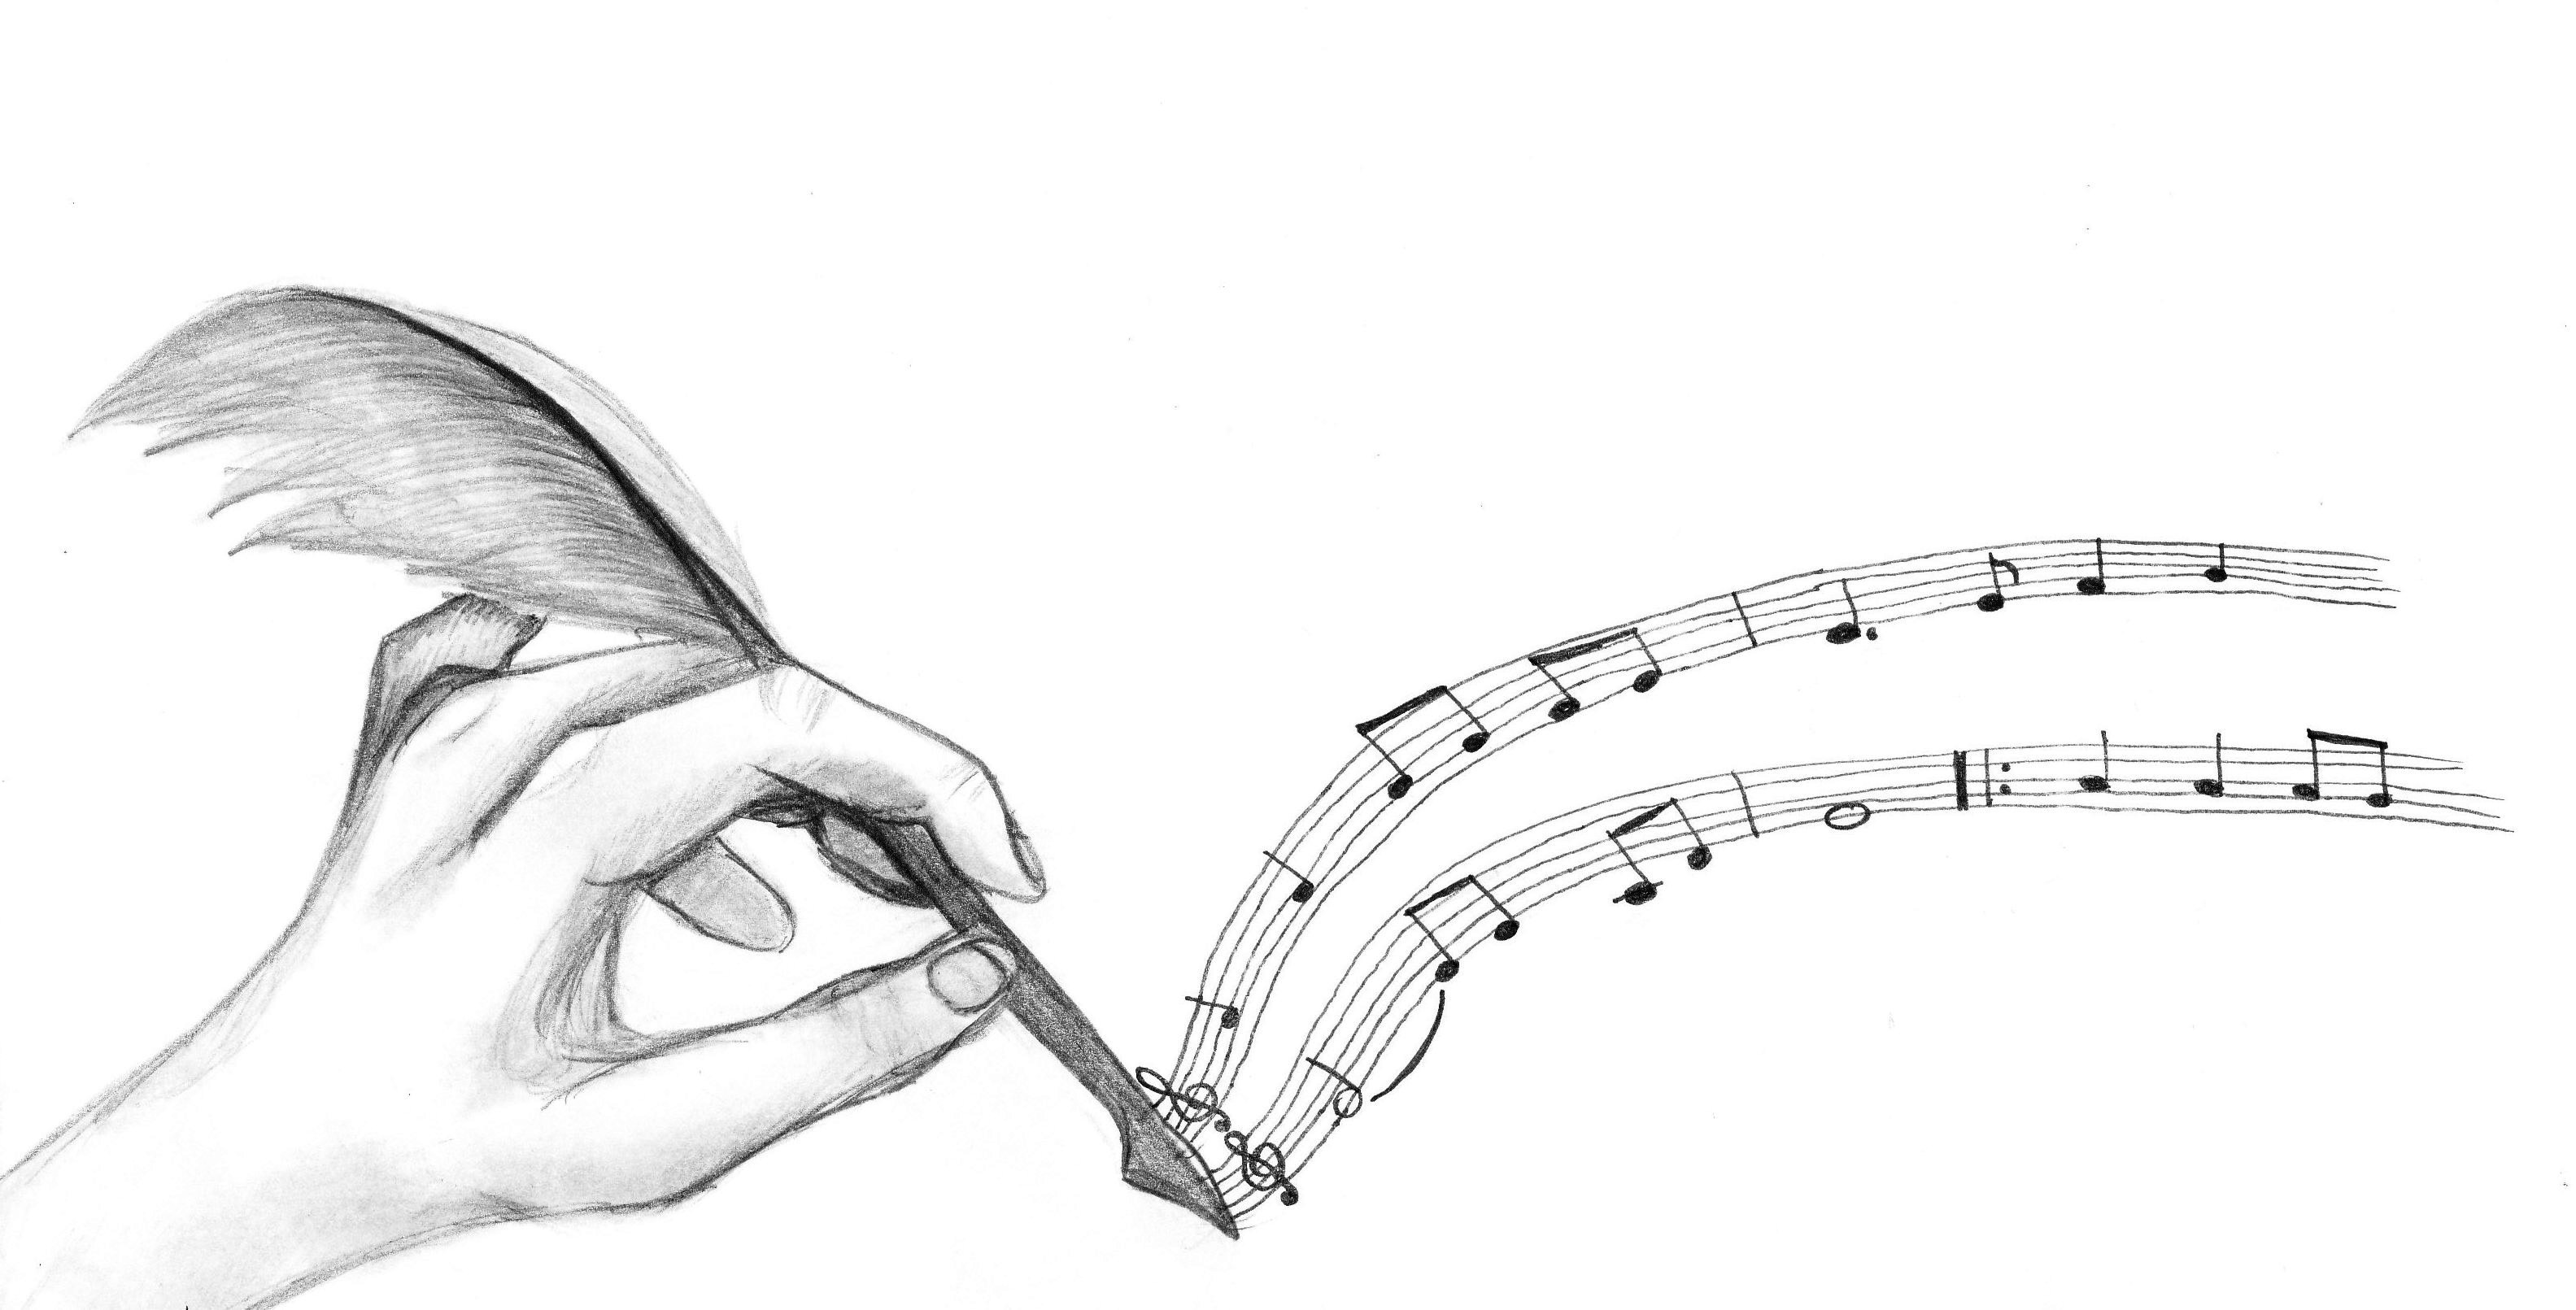
\includegraphics[width=1\textwidth]{Noten/SturmUndDrang.pdf}

% \beginverse
% \[Am]Jeden Morgen ruft das \[Dm]junge Leben, \[Am]was der Tag ihm \[E]bringt.
% \lrep \[Am]Bis der Zweifel all die \[Dm]guten Taten \[Am]schließlich zu \[E]Boden \[Am]ringt. \rrep
% \lrep \[Am]Gestern ist vorbei (Gestern ist vorbei), \[C]Morgen einerlei (Morgen einerlei),
% \[G]Heute noch da sind wir \[Am]jung!\rrep
% \endverse

\beginverse\memorize
\[Am]Irgendwann sucht ihr nach \[Dm]eurem Leben: 
\[Am]Fragt, man hört euch \[E]nicht!
\lrep \[Am]Schon zu lange schirmt des \[Dm]Trübsal Schatten \[Am]euer \[E]Ange\[Am]sicht. \rrep
\endverse

\beginchorus
\lrep \[Am]Gestern ist vorbei \echo{Gestern ist vorbei}, 
\[C]Morgen einerlei \echo{Morgen einerlei},
\[G]Heute noch lacht uns das \[Am]Glück! \rrep
\endchorus

\beginverse
^Drum verlacht die nieder^trächtgen Pfeile, 
^die der Teufel ^schnitzt. 
\lrep ^Handelt stets nach eurem ^eigenen Herzen, ^dass kein ^Pfeil es ^ritzt. \rrep
\endverse

\beginchorus
^Gestern ist vorbei \echo{Gestern ist vorbei}, 
^Morgen einerlei \echo{Morgen einerlei},
^Heute noch da sind wir ^jung!
\[Am]Gestern ist vorbei \echo{Gestern ist vorbei}, 
\[C]Morgen einerlei \echo{Morgen einerlei},
\[G]Heute noch lacht uns das \[Am]Glück!
\endchorus

\endsong
